$subject$=Физические основы компьютерных \\ и сетевых технологий
$teacher$=Лекции Герта А. В.
$date$=07.04.2025

\section{Лекция 9. Интерференция света}

Поляризация света - упорядоченность в ориентации векторов напряженностей электрического поля $E$
и магнитного поля $H$ световой волны в плоскости, перпендикулярной распространению света

Различают: 

\begin{enumerate}
    \item линейную поляризацию света, когда ориентация вектора $E$ сохраняет постоянное направление 
(плоскость, в которой лежит $E$ и световой луч, называются плоскостью поляризации)

    \item эллиптическую поляризацию, при которой конец $E$ в проекции на плоскость, 
    перпендикулярную направлению света, описывает эллипс 

    \item круговою поляризацию, при которой конец $E$ описывает круг
\end{enumerate}

Обычный, естественный свет, например, от солнца, хаотично поляризован - конец $E$ описывает хаотичные фигуры

Интерференция света - нелинейное сложение интенсивностей двух или нескольких световых волн, 
сопровождающееся пространственным перераспределением энергии светового излучения

Если через точку проходят две волны с векторами $\vec E_1$ и $\vec E_2$, то в точке напряженность равна $E = E_1 + E_2$, 
а интенсивность света определяется так: $\langle \vec E^2 \rangle = \langle \vec E_1^2 \rangle + \langle \vec E_2^2 \rangle + 2\langle (\vec E^2_1, \vec E_2^2) \rangle$

Если $2\langle (\vec E^2_1, \vec E_2^2) \rangle = 0$, то интерференции нет, если $2\langle (\vec E^2_1, \vec E_2^2) \rangle \neq 0$, то есть 

В частности, если $E_1 \perp E_2$, то интерференции нет 

При этом интенсивность света в точке равна $I = I_1 + I_2 + 2\sqrt{I_1 I_2} \cos \langle \delta \rangle$, где $\langle \delta \rangle$ - разность фаз

Нарушение аддитивности интенсивности связано не с нарушением ЗСЭ, а с перераспределением энергии 
по волновому фронту при взаимодействии волн

Если разность фаз колебаний в точке постоянна, то есть $\langle \delta \rangle = \delta (r_1, r_2)$, то колебания и волны называют когерентными

Чтобы две световые синусоидальные волны были когерентными, их частоты должны быть одинаковыми.
Слагаемое $2\sqrt{I_1 I_2} \cos \langle \delta \rangle$ называют интерференционным членом

\mediumvspace

Рассмотрим два точечным источника света, которые описывают интерференционную картину на экране

\smallvspace

% https://www.geogebra.org/calculator/cbg9buf2

\begin{center}
    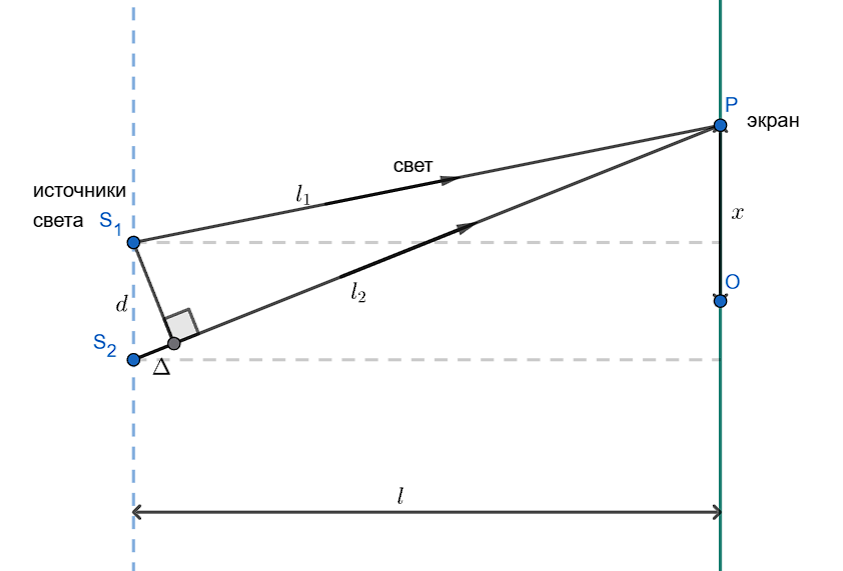
\includegraphics[width=0.75\textwidth]{physics2/images/physics2_2025_04_07_1}
\end{center}

\smallvspace

Величина $l = ns$, где $n$ - показатель преломления, называется оптической длиной пути, 
величина $\Delta \equiv l_1 - l_2$ - оптической разностью пути

Если $\Delta = n \frac{x d}{l} = m \lambda_0$ ($m \in \Integer$), то $\cos \delta = \cos 2\pi m = 1$, свет будет в одной фазе 
и в точке будет наблюдаться максимум интенсивности

А если $\Delta = \frac{2m + 1}{2} \lambda_0$, то будет наблюдаться минимум

В общем, на экране будет наблюдаться картина, состоящая из темных и светлых полос. Светлые полосы отображают
максимумы, а темные - минимумы

Если свет пропустить через решетку с тоненькими прорезями, то излучаемый оттуда свет можно считать точечными источникам.
И на экране получается картина из светлых и темных полос. Явление света огибать решетку получило название дифракция

